\chapter{系统实现和工具演示}

\section{\wa 系统实现}

\wa 在实验评估中使用 Java 语言实现,并使用 Apache POI 库 \footnote{https://poi.apache.org} 来读写 Excel 格式的电子表格,由于包含一些历史遗留的 DLL 文件,目前只能在 Windows 操作系统下执行。
相应源码发布在 GitHub 网站上 \footnote{https://github.com/dlee992/QRS19-Code} 。

\wa 工具总共包含约 7,300 行 Java 代码,除了包含 \cu 的源代码以外,额外增改了约 2,500 行代码。
类似于 \cu 的方式,\wa 标记它分析过的电子表格的方法是使用不同的背景色来标注检测到的同一张工作表内的所有单元格类,并通过在单元格右上角添加注释的方式标注该单元格的缺陷类型,例如丢失公式的缺陷或者包含不一致公式的缺陷。

\section{SGuard 集成化测试工具}

\sg 工具也是使用 Java 实现的独立于 Excel 的可视化集成工具,也是用 Apache POI 库来读写 Excel 格式的电子表格。
和\wa 类似,目前只能在 Windows 操作系统下执行。
\sg 的初始核心代码是由张瑞青开发的,我们额外添加了两个新技术模块,即 \cu-OPT 和 \wa ,并进行了对应的集成编码工作\cite{li2019sguard}。
相应的工具介绍主页发布在 GitHub Pages 上 \footnote{https://sheetguard.github.io/sguard/},其中包含了工具源码链接和介绍性的视频链接,发布在 YouTube \footnote{https://www.youtube.com/watch?v=gNPmMvQVf5Q} 和 Bilibili 网站上。

\sg 的完整实现包含约 10,500 行 Java 代码,其中包含 7,300 行核心代码和 3,200 行图形界面代码。

\subsection{界面设计}

\begin{figure}[tbp]    
    \centering
    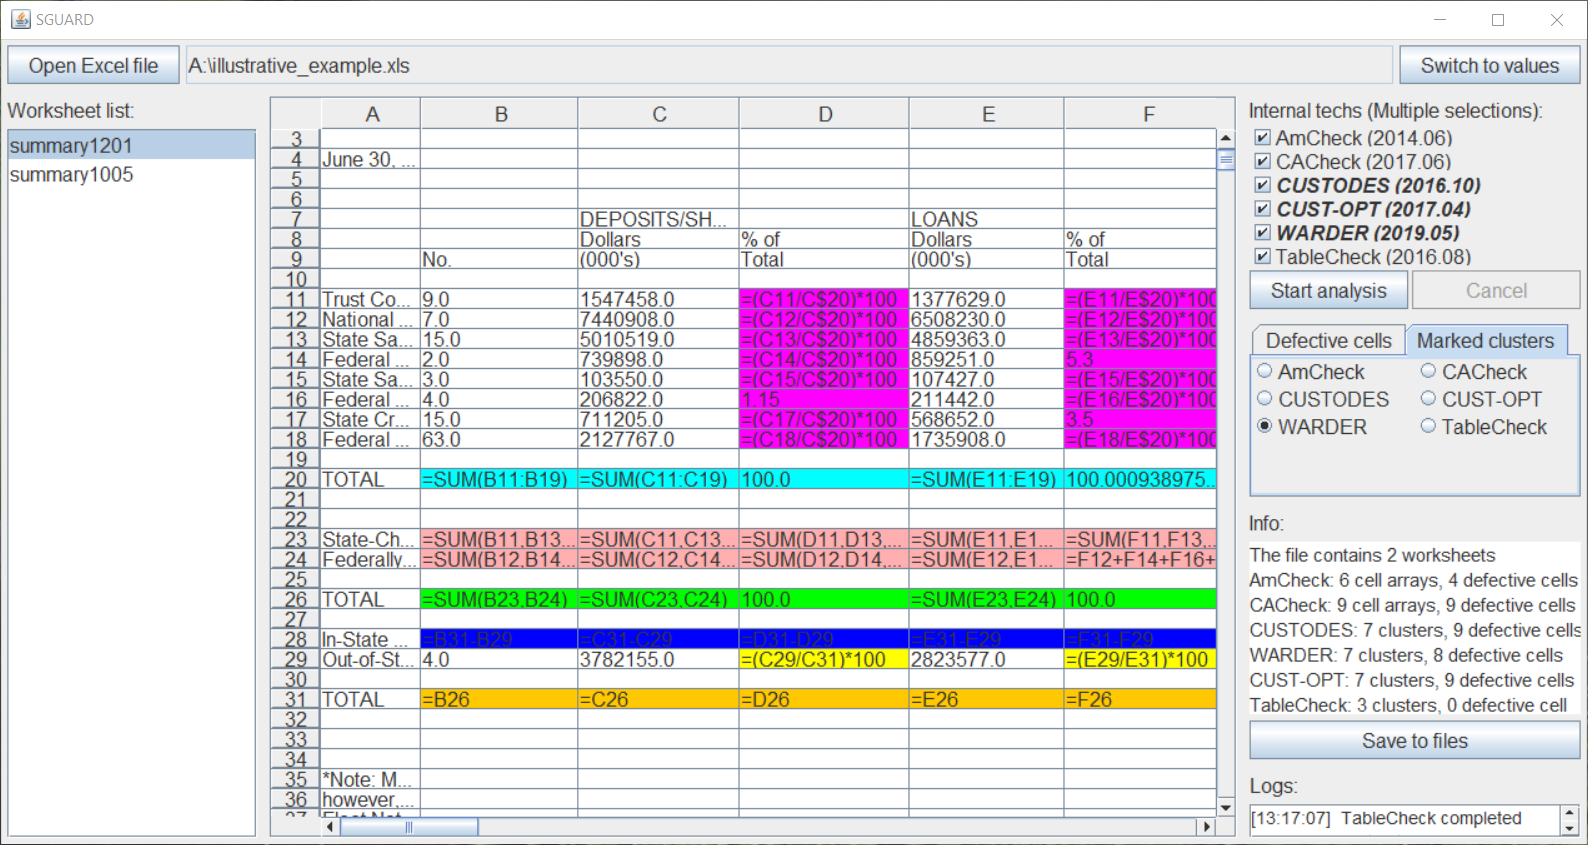
\includegraphics[width=\textwidth]{figure/figure11.png}
    \caption{\sg 的使用截图}
    \label{figure11}
\end{figure}

图\ref{figure11} 展示了\sg 使用交互界面来检测电子表格并展示相应结果的截图。
整个界面包含四大区域:

\begin{itemize}
    \item 上方的文件选取区域包含 Open Excel file(打开 Excel 文件)和Switch to values/formulas(切换到数值/公式形式)两个按钮,中间部分显示当前打开的 Excel 文件路径,如 A:$\backslash$illustrative\_exmaple.xls;
    \item 左侧的工作表选择区域列出了当前选定的 Excel 文件的所有工作表;
    \item 中间的工作表内容展示区域展示了类似于电子表格软件的核心界面,以字母标记的列号(A,B,\dots)和以数字标记的行号(1,2,\dots),每个对应的表格位置显示该工作表的具体内容,即公式,数值或文本,目前不能显示除此以外的模块,比如工作表中插入的图,以及不会保留原工作表的排版风格,只显示每个单元格里的具体内容(特别地,还不支持显示多单元格合并为一个单元格的显示效果);
    \item 右侧的核心操作区域包含如下几块内容:
        \begin{enumerate}
            \item 上方罗列了 \sg 工具内部囊括的所有检测技术,共有 6 个检测技术,分别是 \am\cite{dou2014spreadsheet},\ca\cite{dou2017cacheck},\cu\cite{cheung2016custodes},\cu-OPT\footnote{http://sccpu2.cse.ust.hk/custodes/cc2s.html},\wa\cite{li2019sguard} 和 TableCheck\cite{dou2016detecting}。每个技术名称后面标记了对应论文发表的时间或者该技术更新的最新时间;
            \item 紧接着向下是 Start analysis 和 Cancel 两个按钮,顾名思义,分别用来开始执行技术对应的代码和取消当前分析过程;
            \item 再往下有两个显示标签,Detective cells 和 Marked clusters,每个运行的技术分别对应一个选项;
            \item 再往下是 Info 栏,展示一些执行信息以及每个电子表格缺陷检测结果汇总,包含每个技术检测到的单元格类数量和有缺陷的单元格数量;
            \item 紧接着是一个 Save to files 按钮,可以用来保存当前选定技术的检测结果到新的 Excel 文件中;
            \item 最后是 Logs 栏,用来显示每个完成执行的技术和对应的时间戳。
        \end{enumerate}
\end{itemize}

\subsection{使用展示}

接下来,我们结合一个简单的工作表例子来展示\sg 的完整使用流程。

\begin{figure}[tbp]    
    \centering
    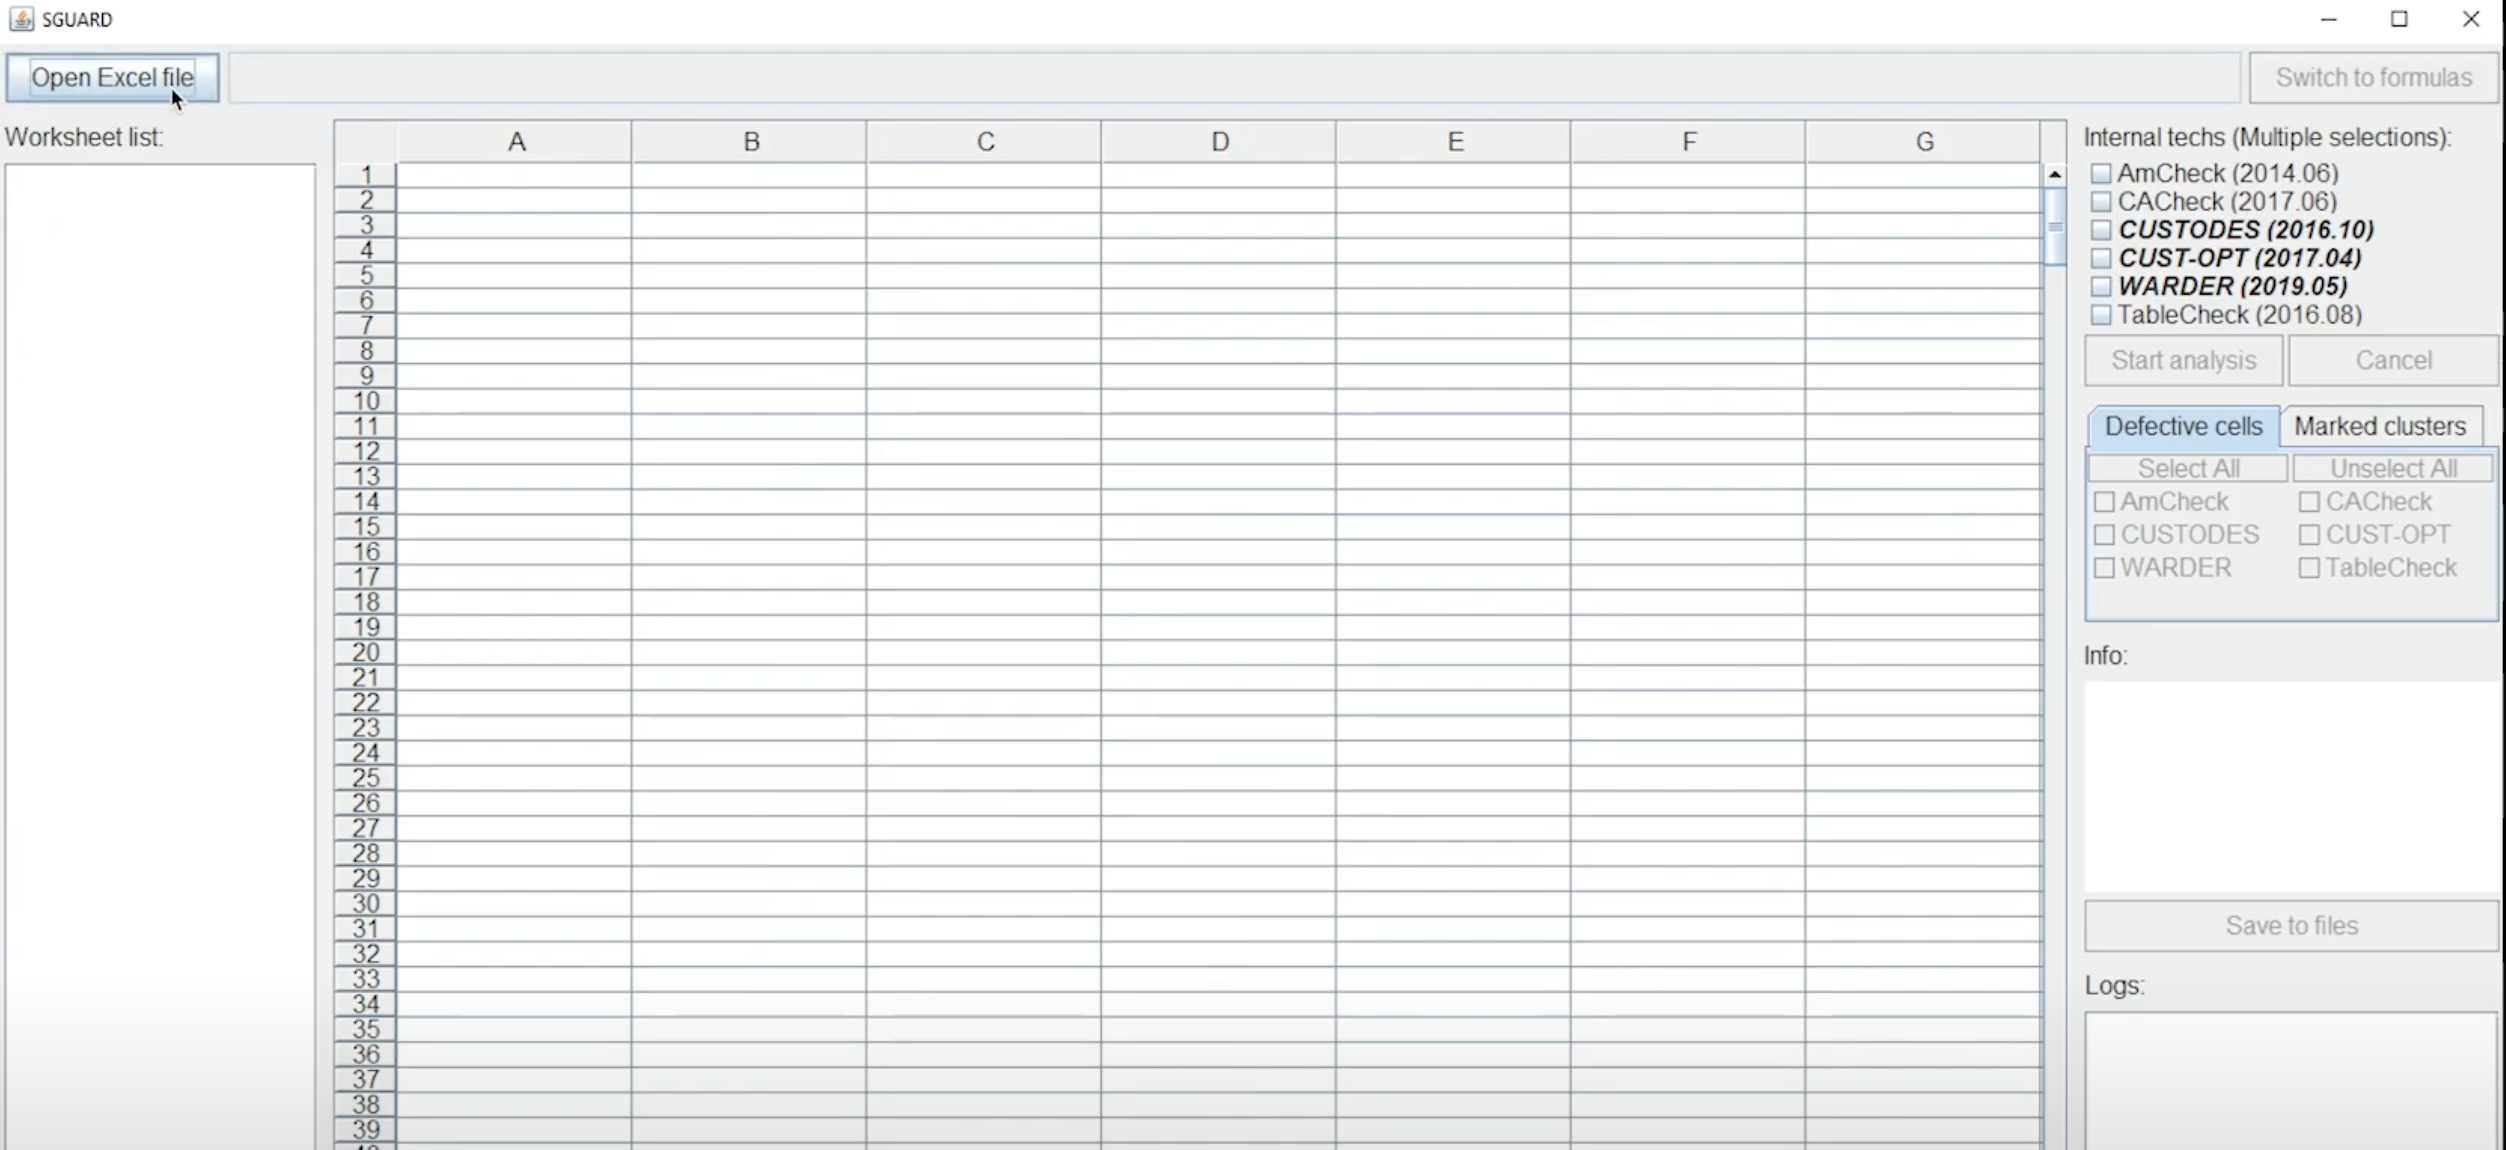
\includegraphics[width=\textwidth]{figure/sg/sguard-1.png}
    \caption{\sg 的使用流程演示截图 1}
    \label{figure-sg1}
\end{figure}
\begin{figure}[tp]   
    \centering
    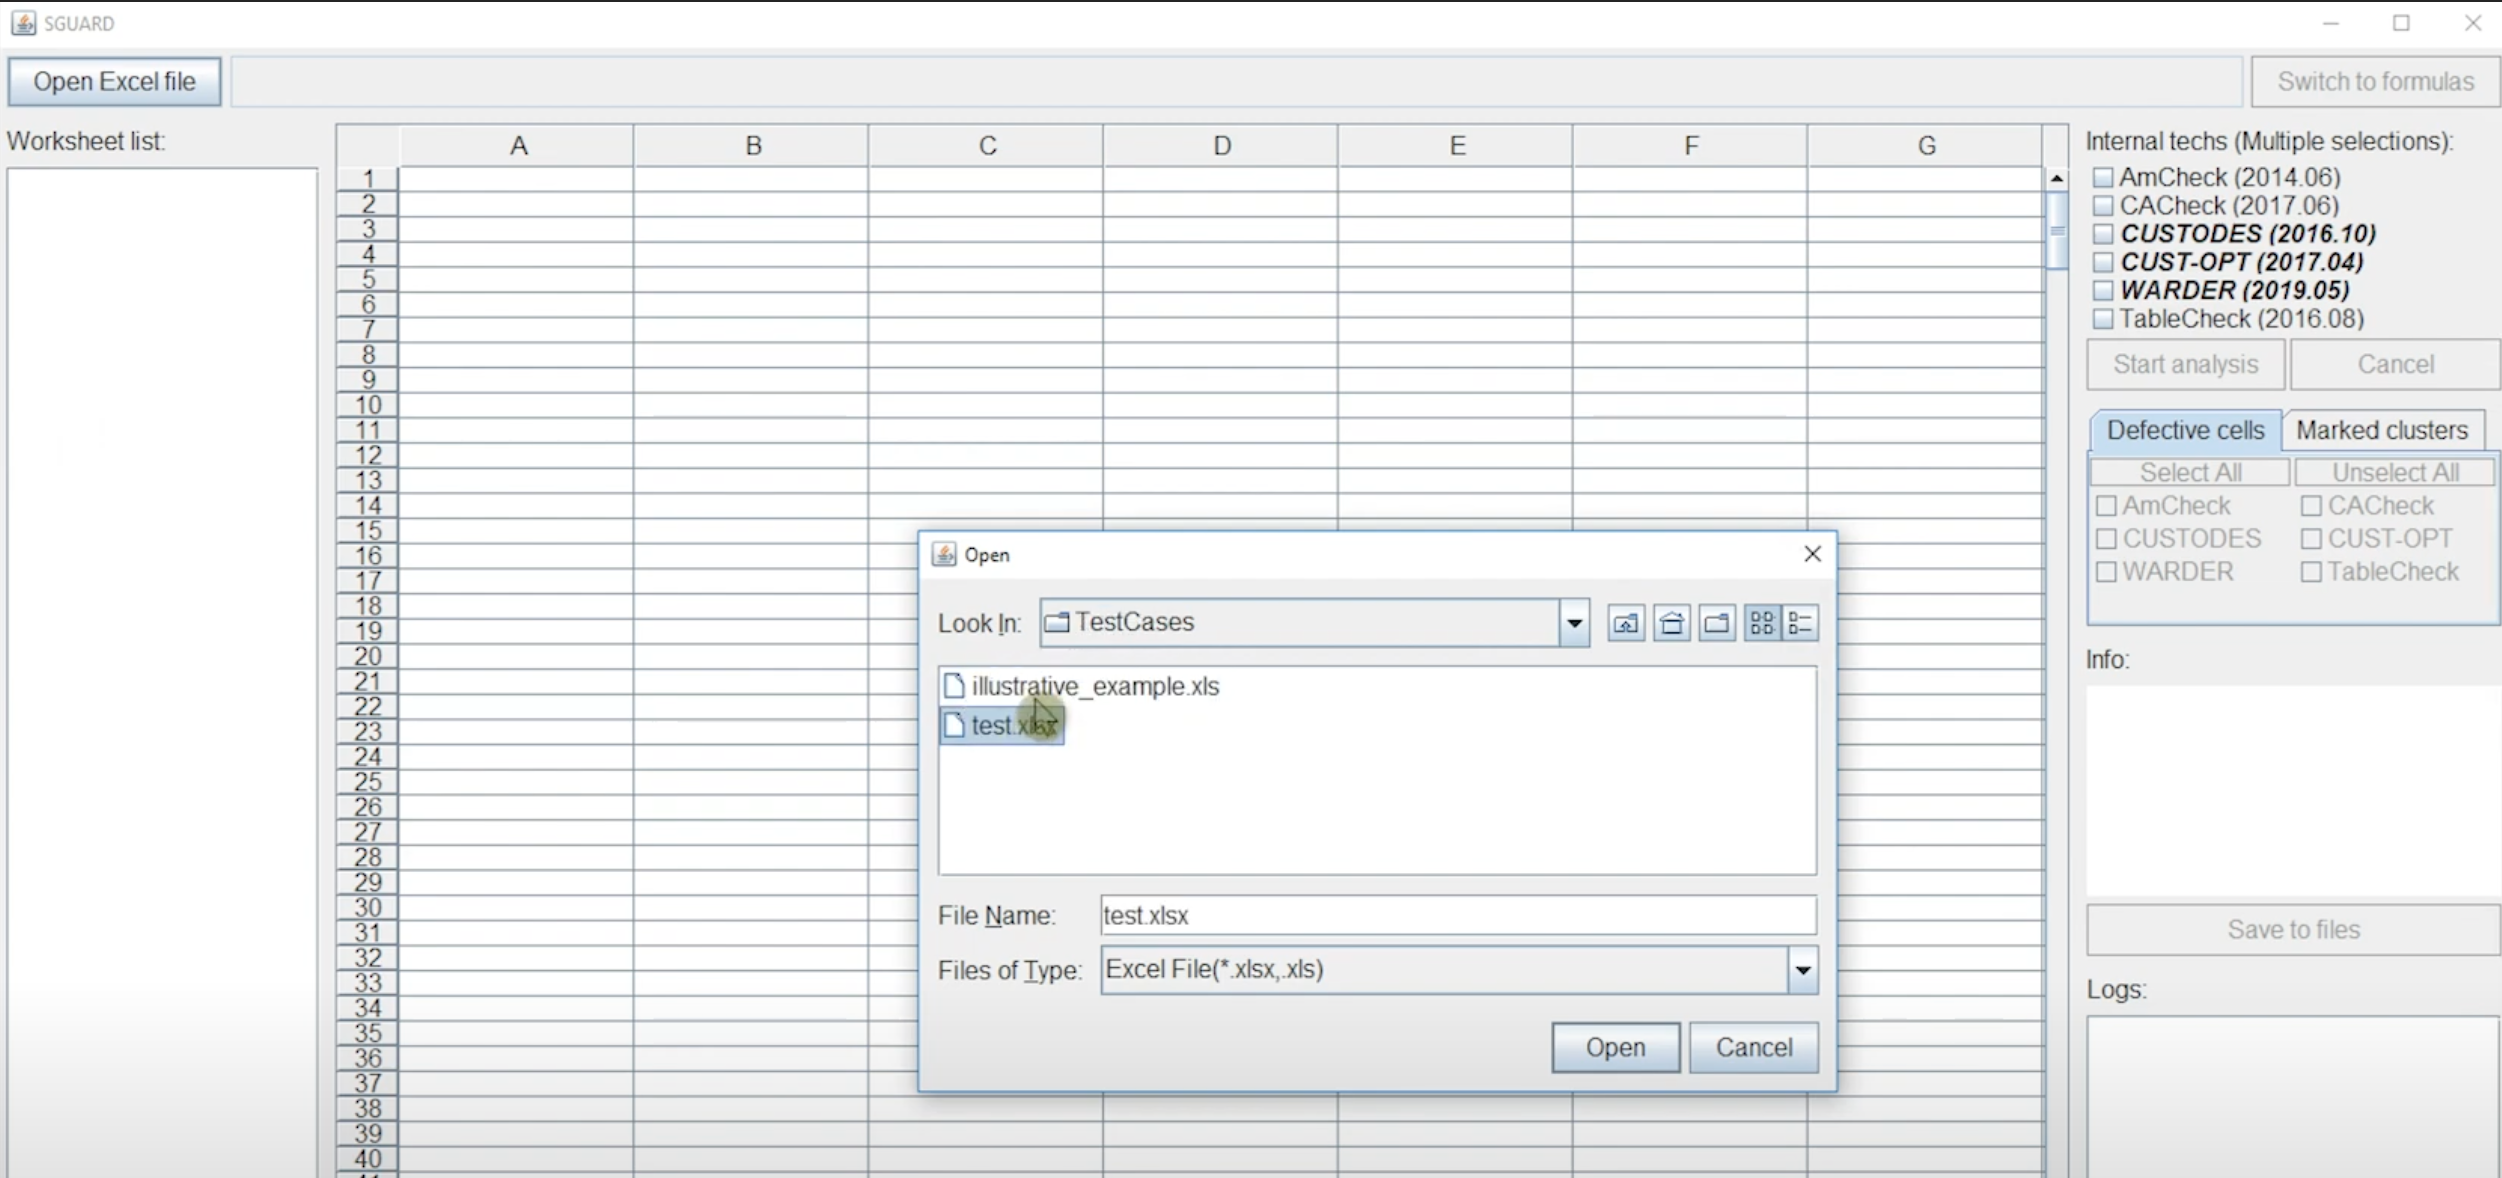
\includegraphics[width=\textwidth]{figure/sg/sguard-2.png}
    \caption{\sg 的使用流程演示截图 2}
    \label{figure-sg2}
\end{figure}
\begin{figure}[tbp]    
    \centering
    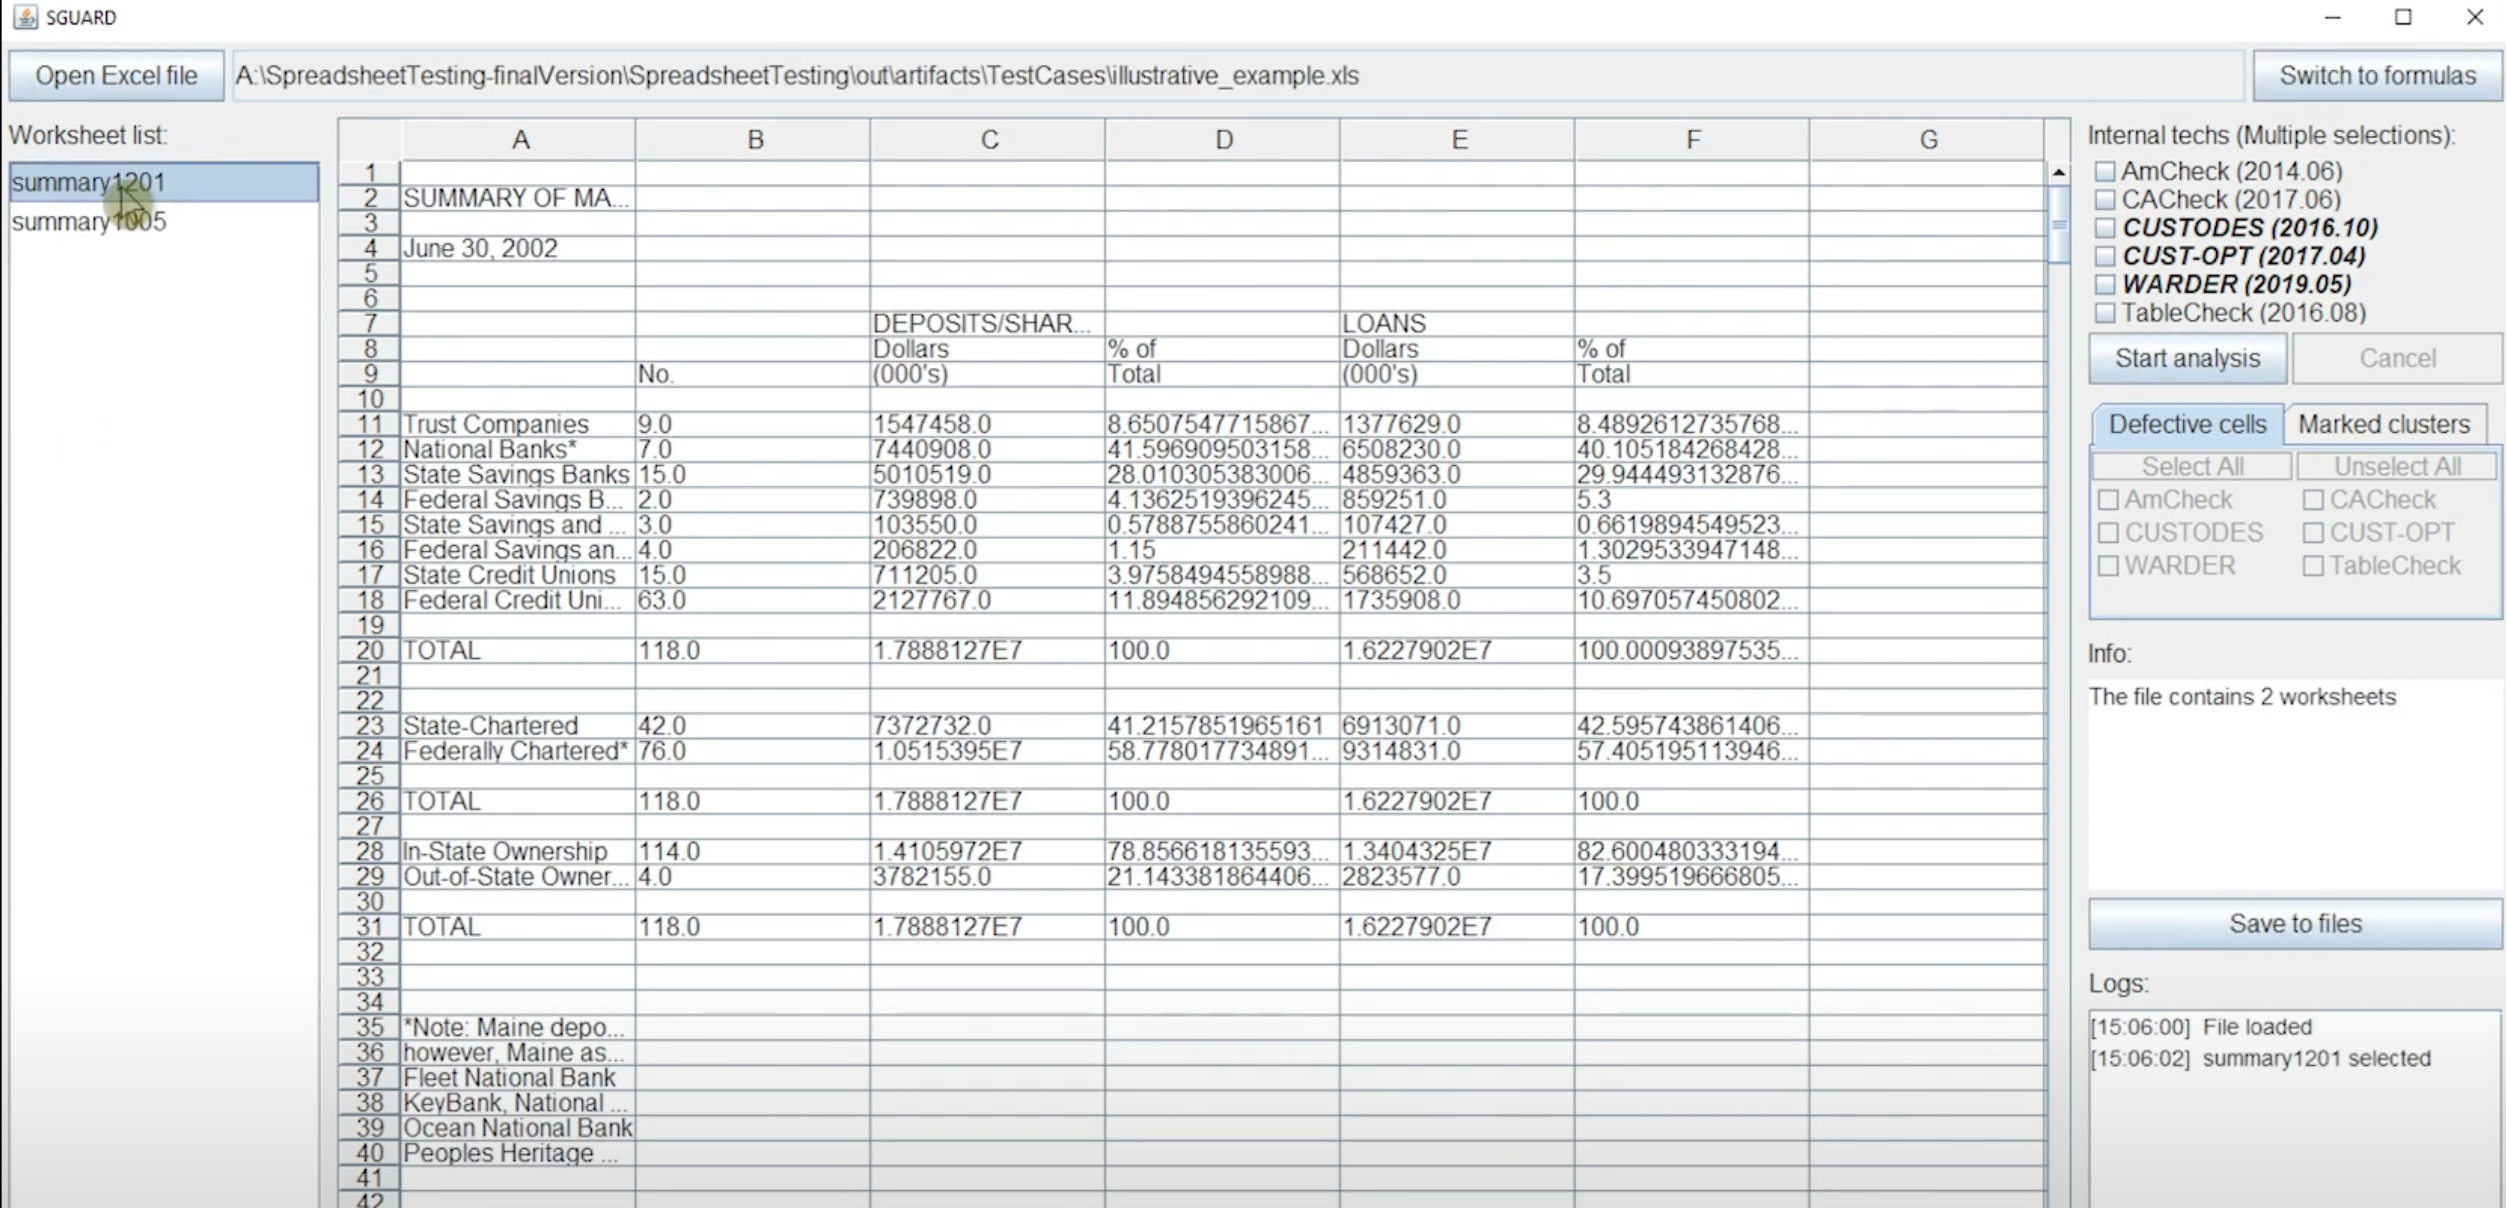
\includegraphics[width=\textwidth]{figure/sg/sguard-3.png}
    \caption{\sg 的使用流程演示截图 3}
    \label{figure-sg3}
\end{figure}
\begin{figure}[tbp]    
    \centering
    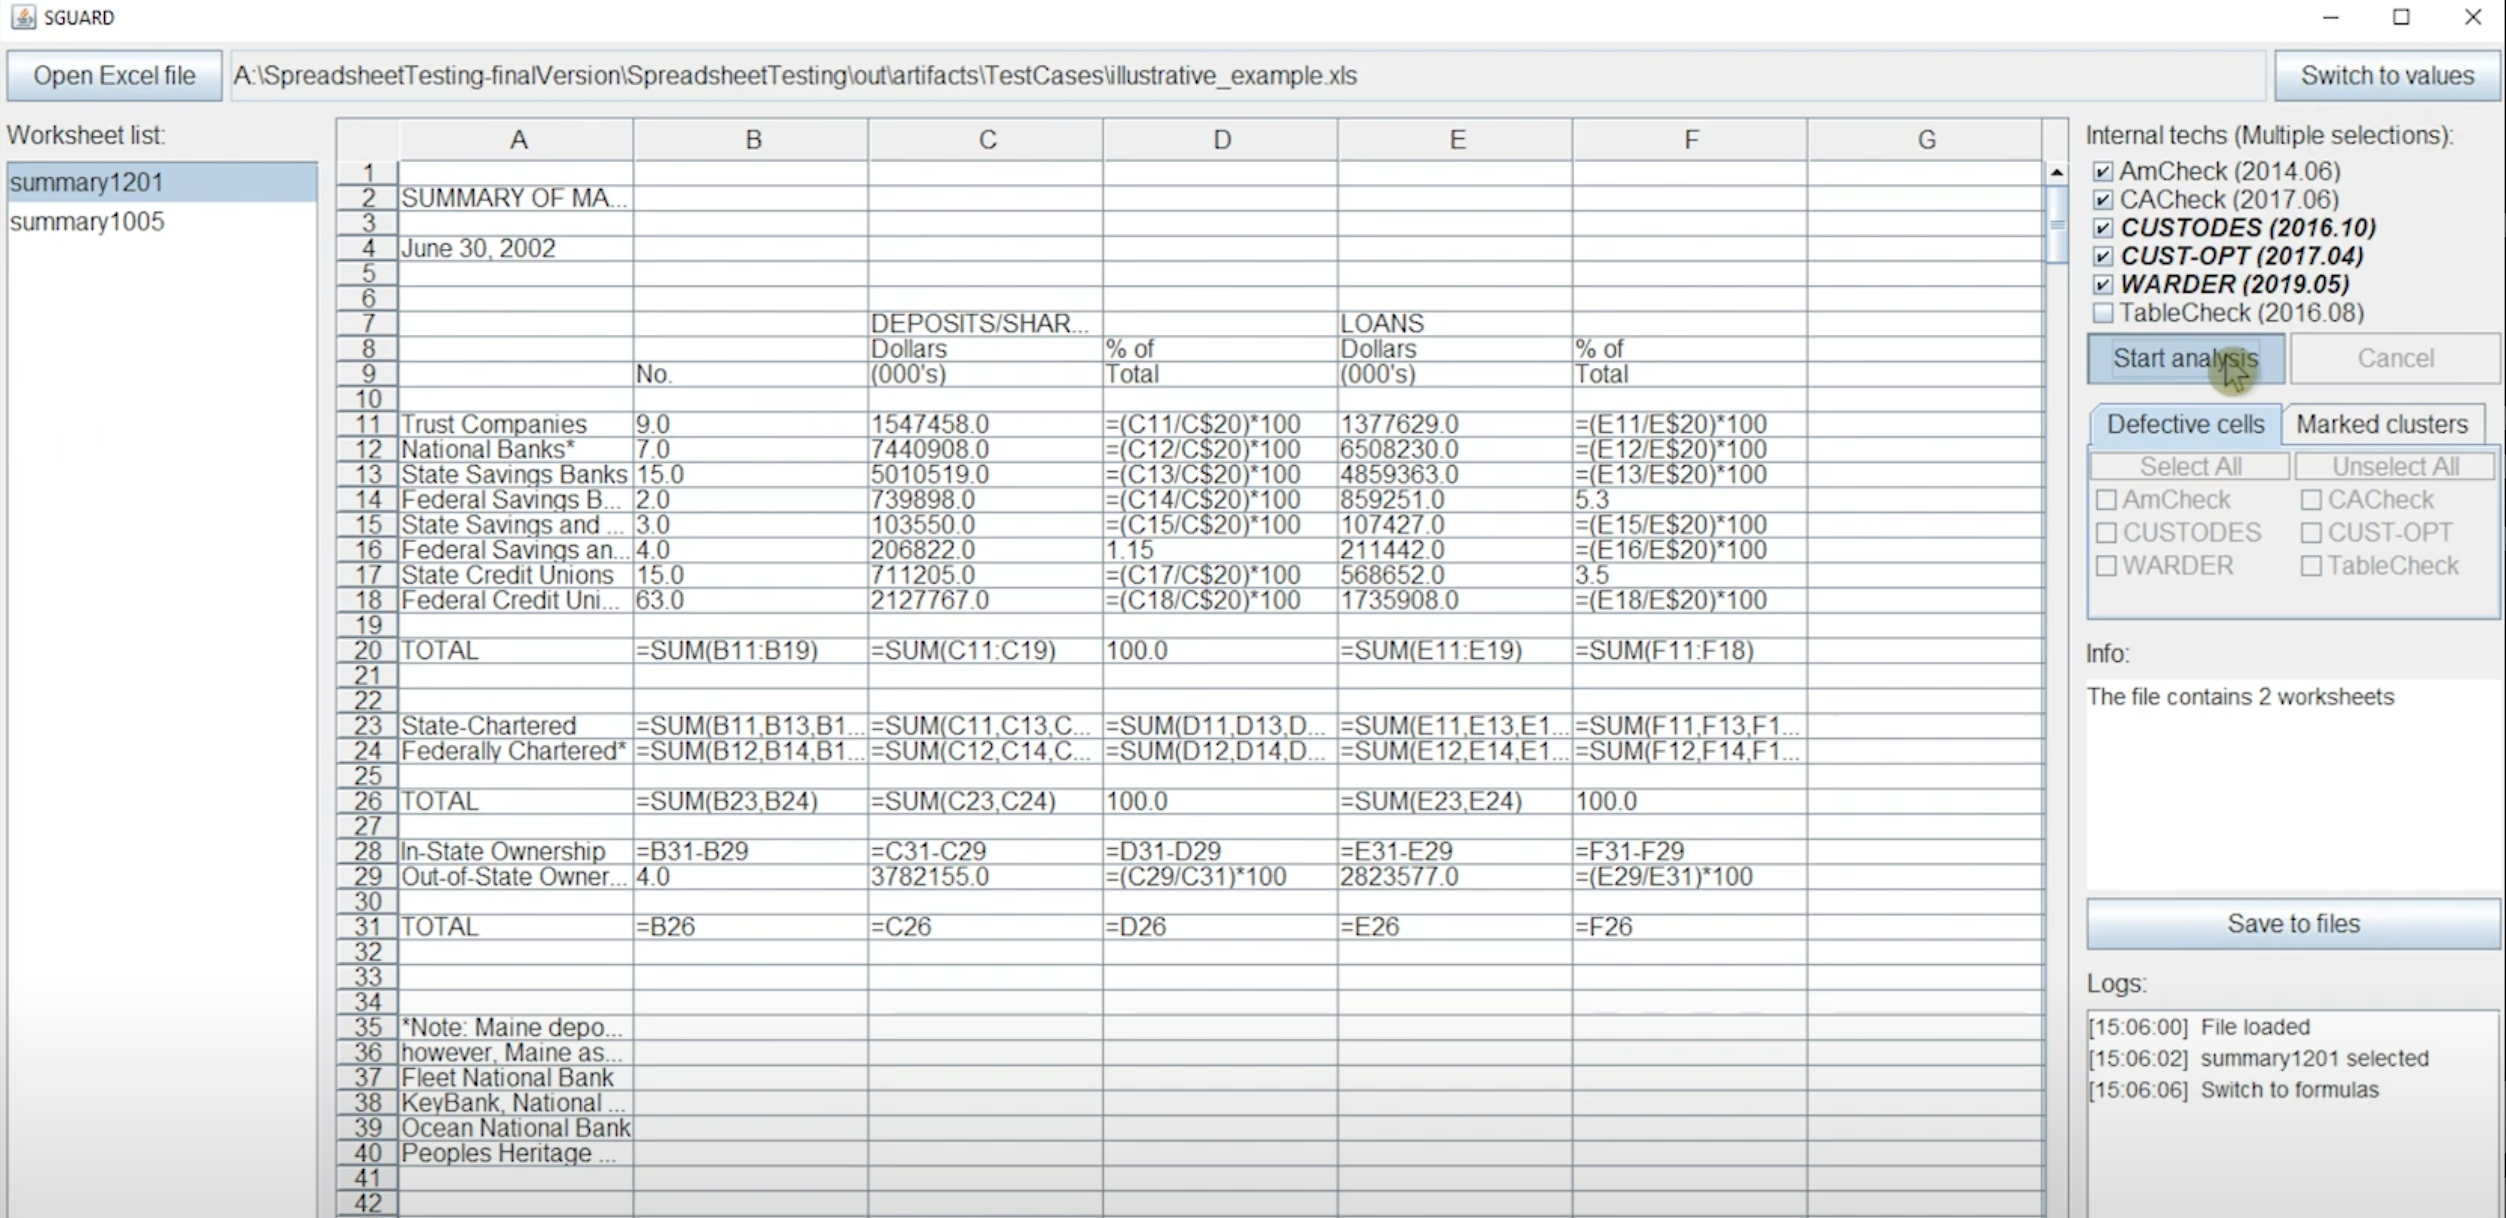
\includegraphics[width=\textwidth]{figure/sg/sguard-4.png}
    \caption{打开待测电子表格并选择待测工作表,再选择要执行的缺陷检测技术并开始执行}
    \label{figure-sg4}
\end{figure}
\begin{figure}[tbp]    
    \centering
    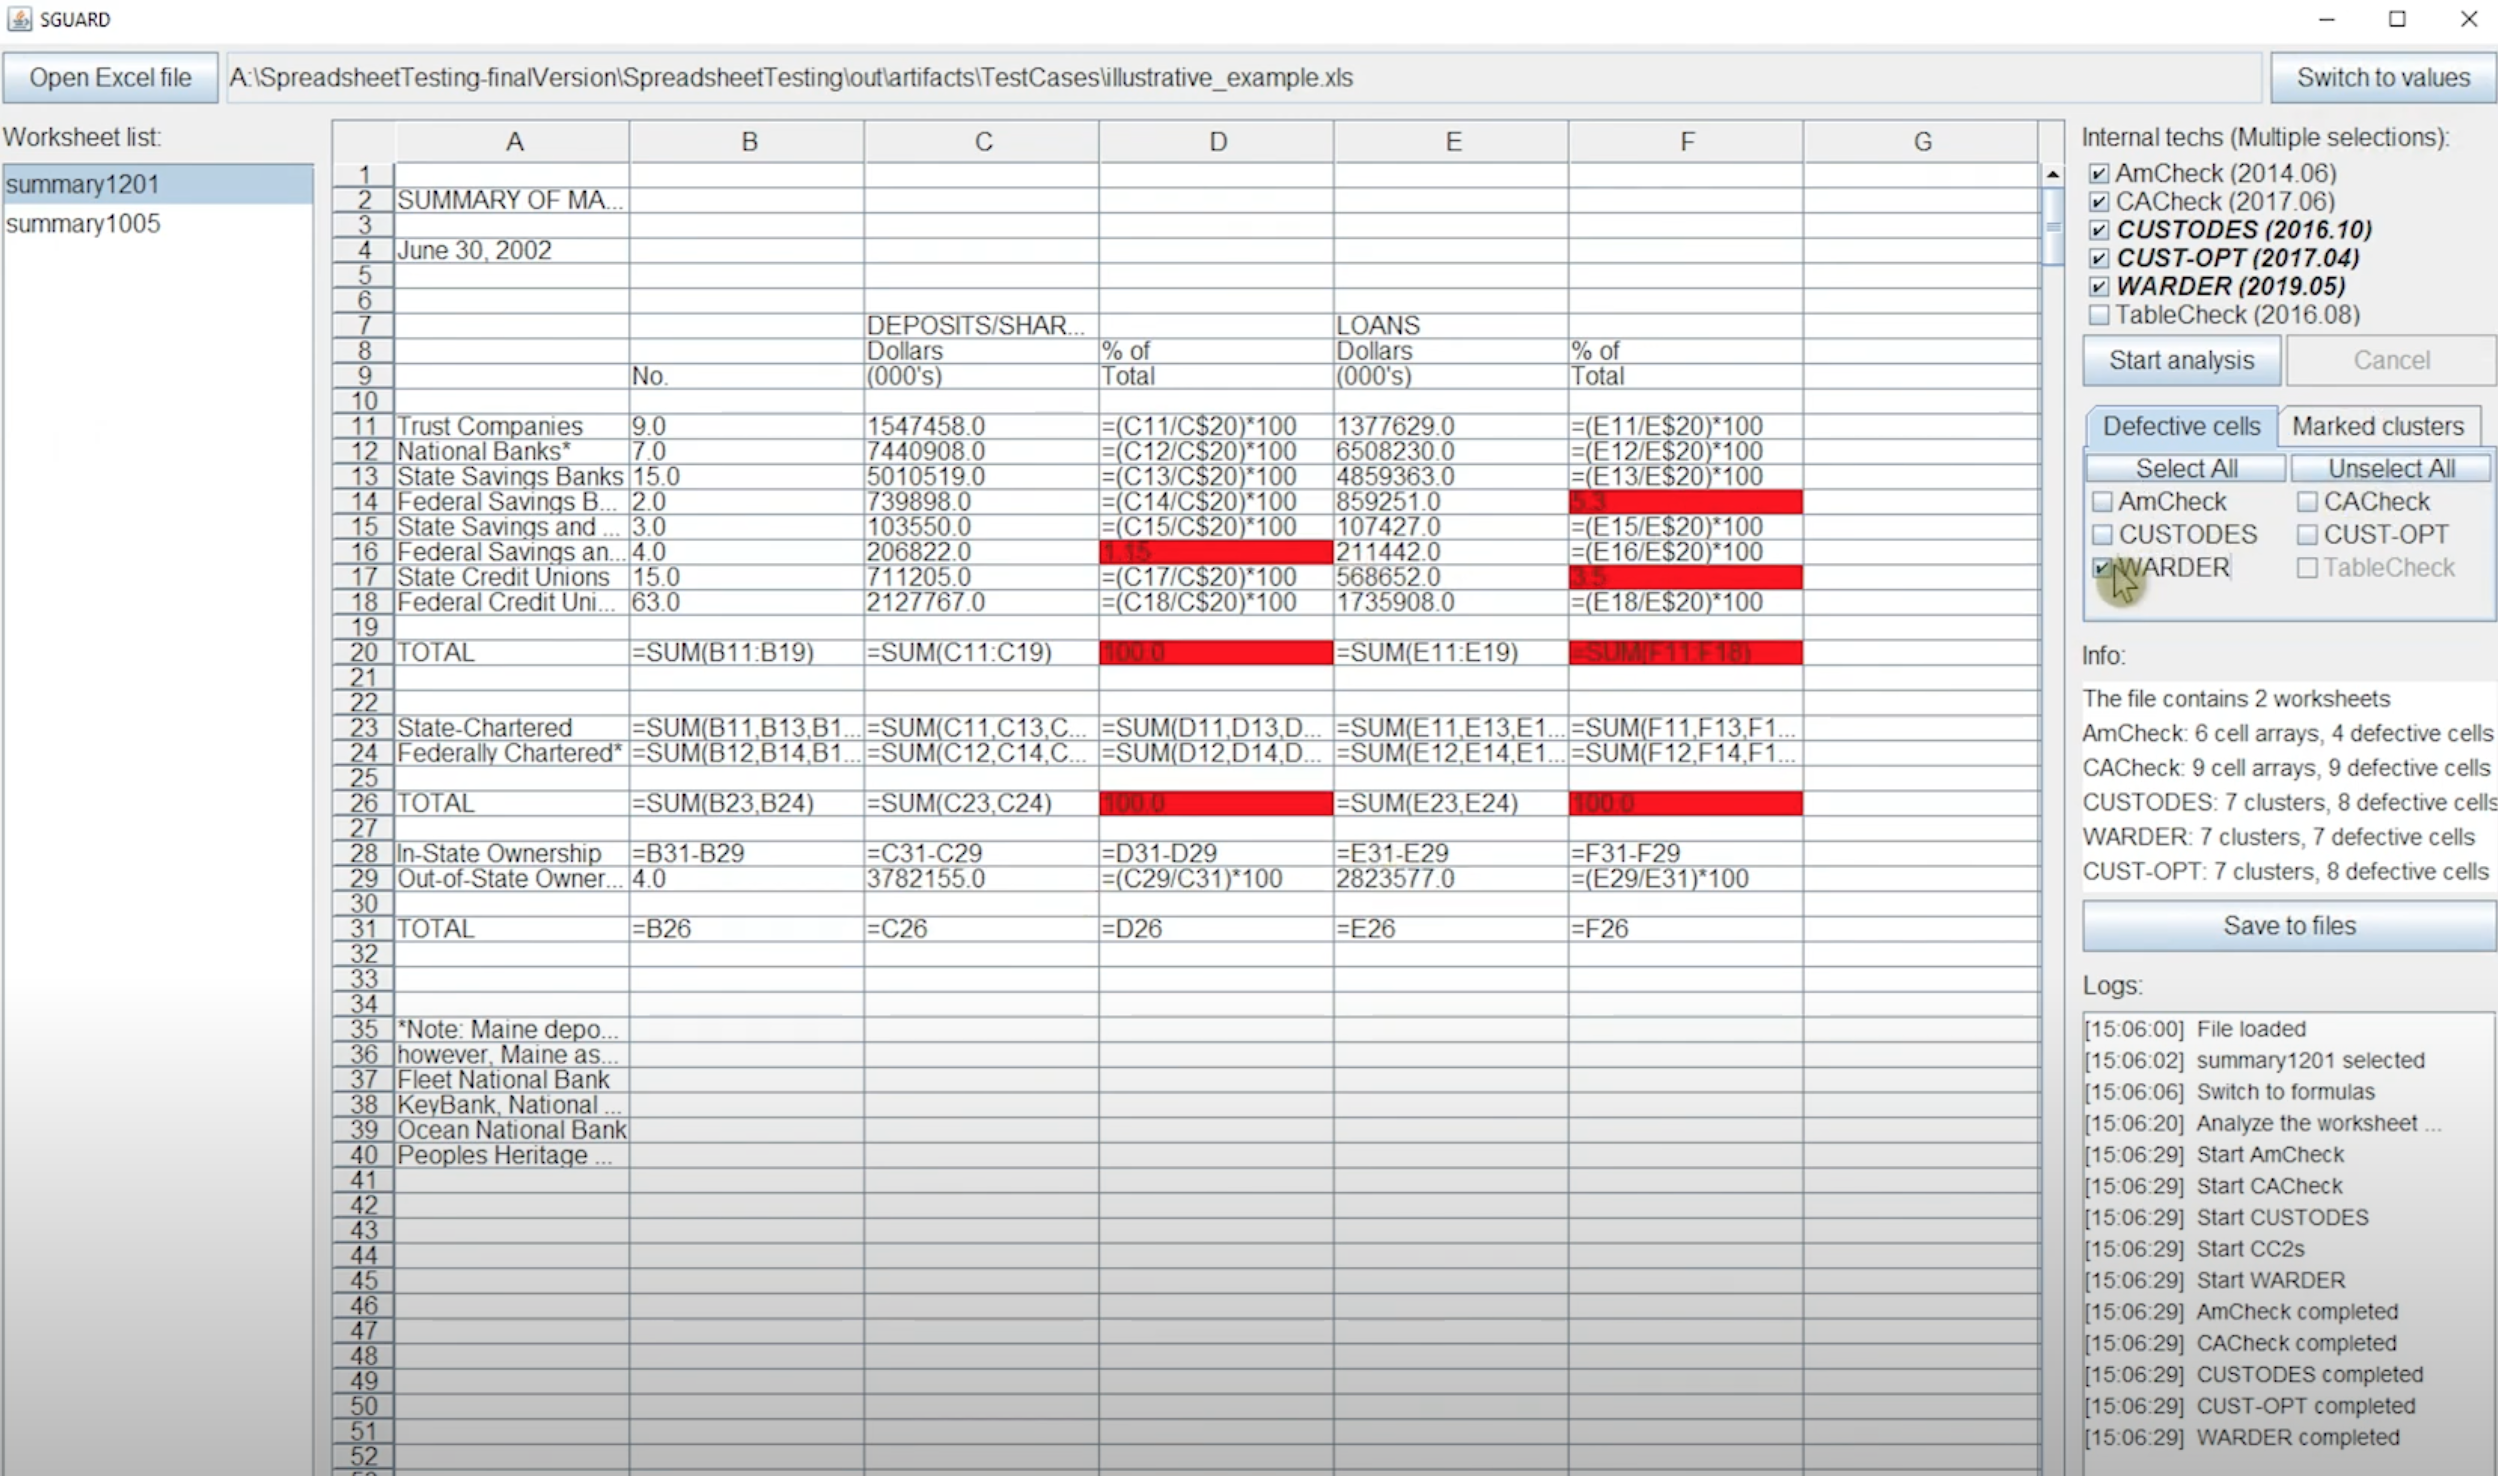
\includegraphics[width=\textwidth]{figure/sg/sguard-5.png}
    \caption{\sg 的使用流程演示截图 5}
    \label{figure-sg5}
\end{figure}
\begin{figure}[tbp]    
    \centering
    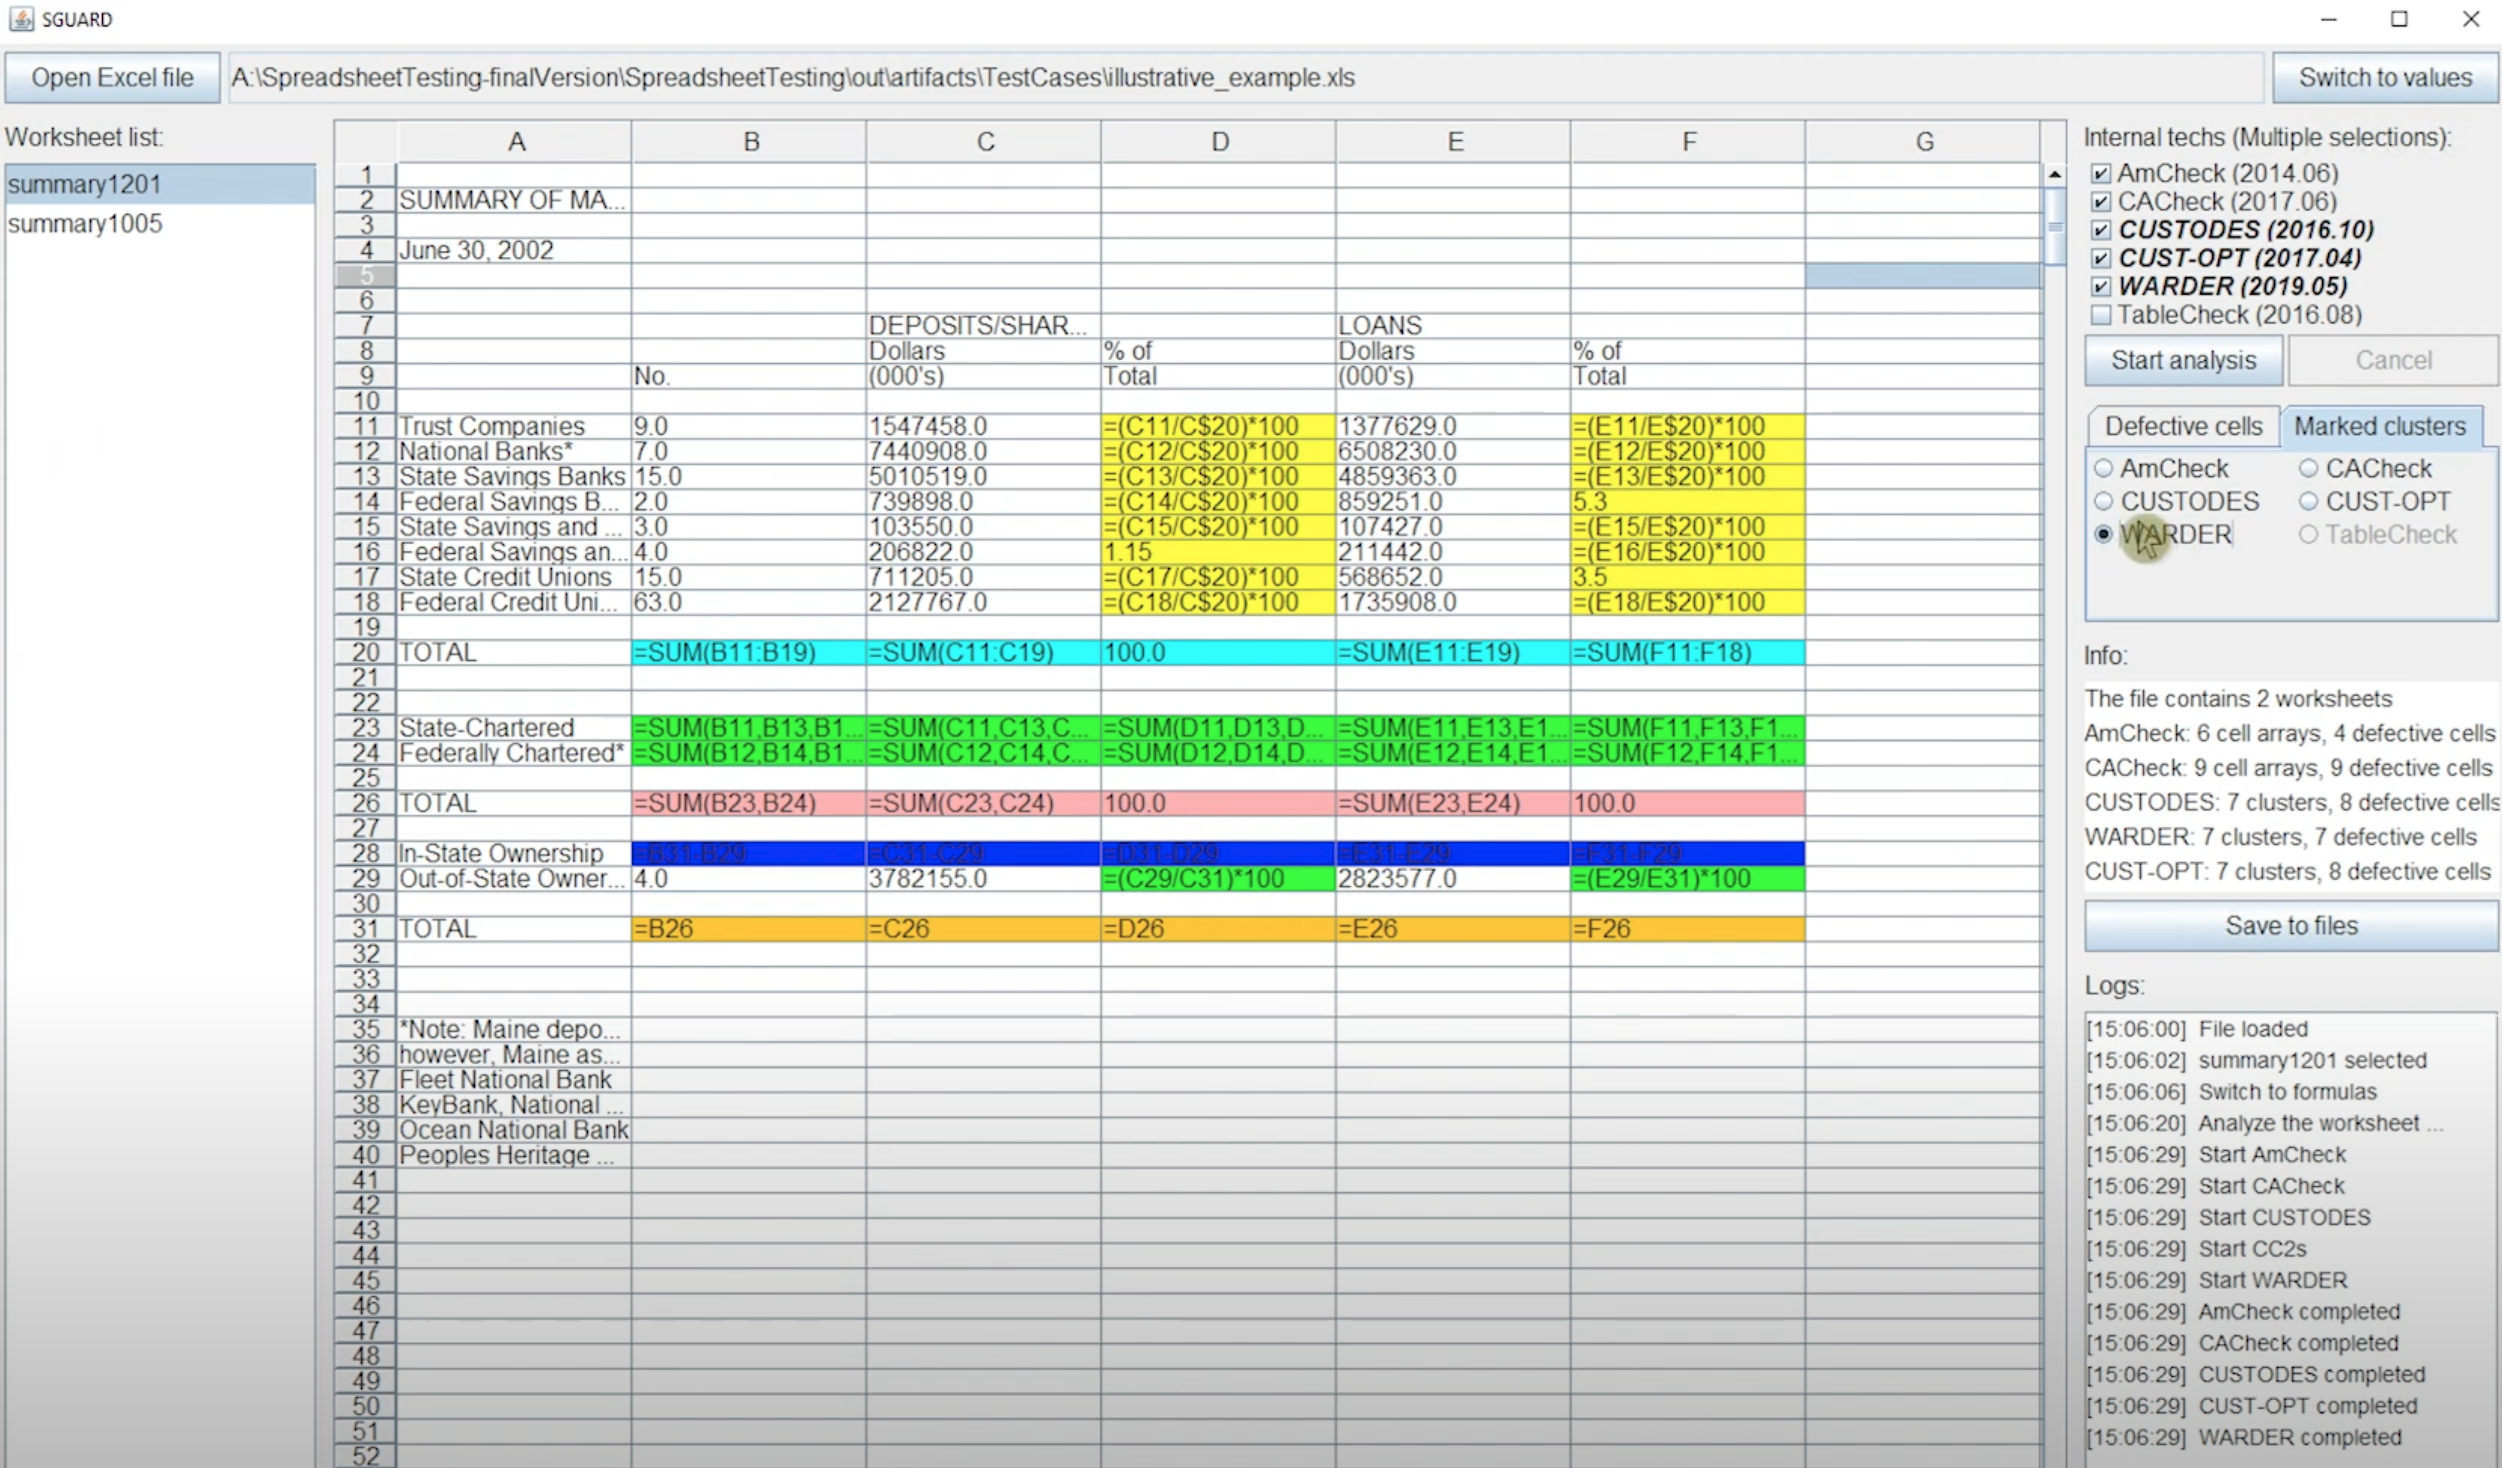
\includegraphics[width=\textwidth]{figure/sg/sguard-6.png}
    \caption{查看 \wa 技术的单元格聚类结果}
    \label{figure-sg6}
\end{figure}
\begin{figure}[tp]    
    \centering
    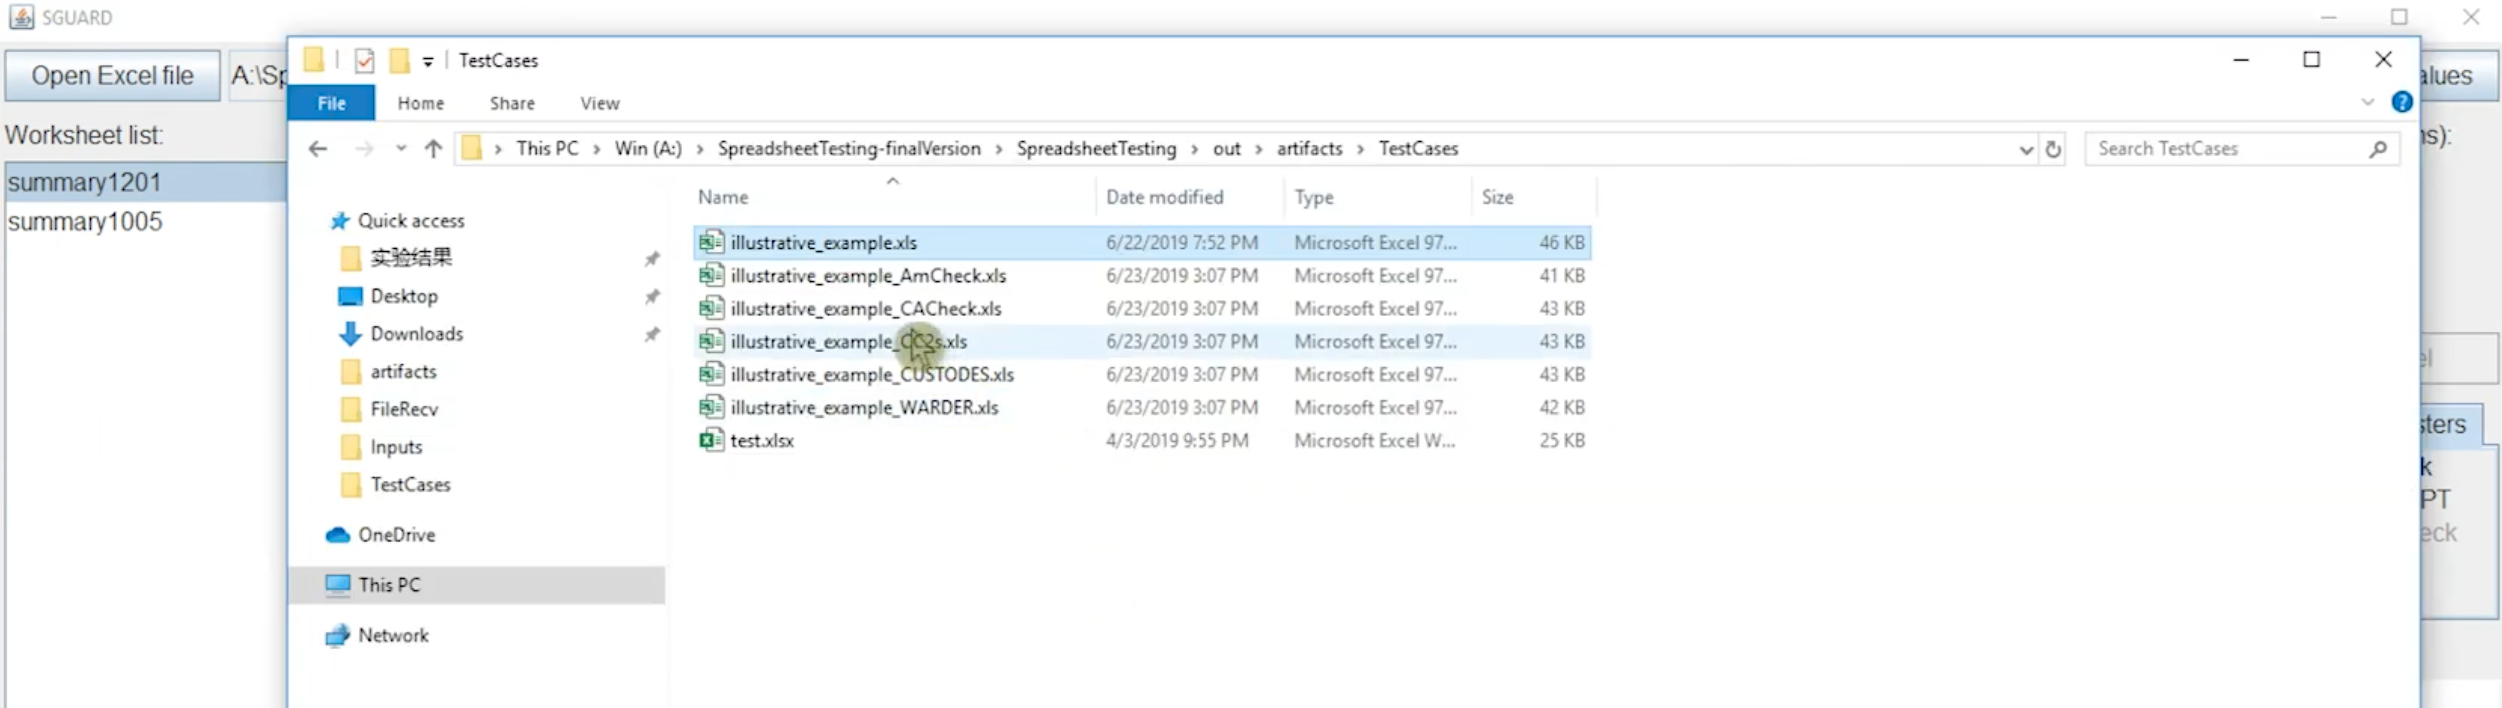
\includegraphics[width=\textwidth]{figure/sg/sguard-7.png}
    \caption{\sg 的使用流程演示截图 7}
    \label{figure-sg7}
\end{figure}
\begin{figure}[tp]    
    \centering
    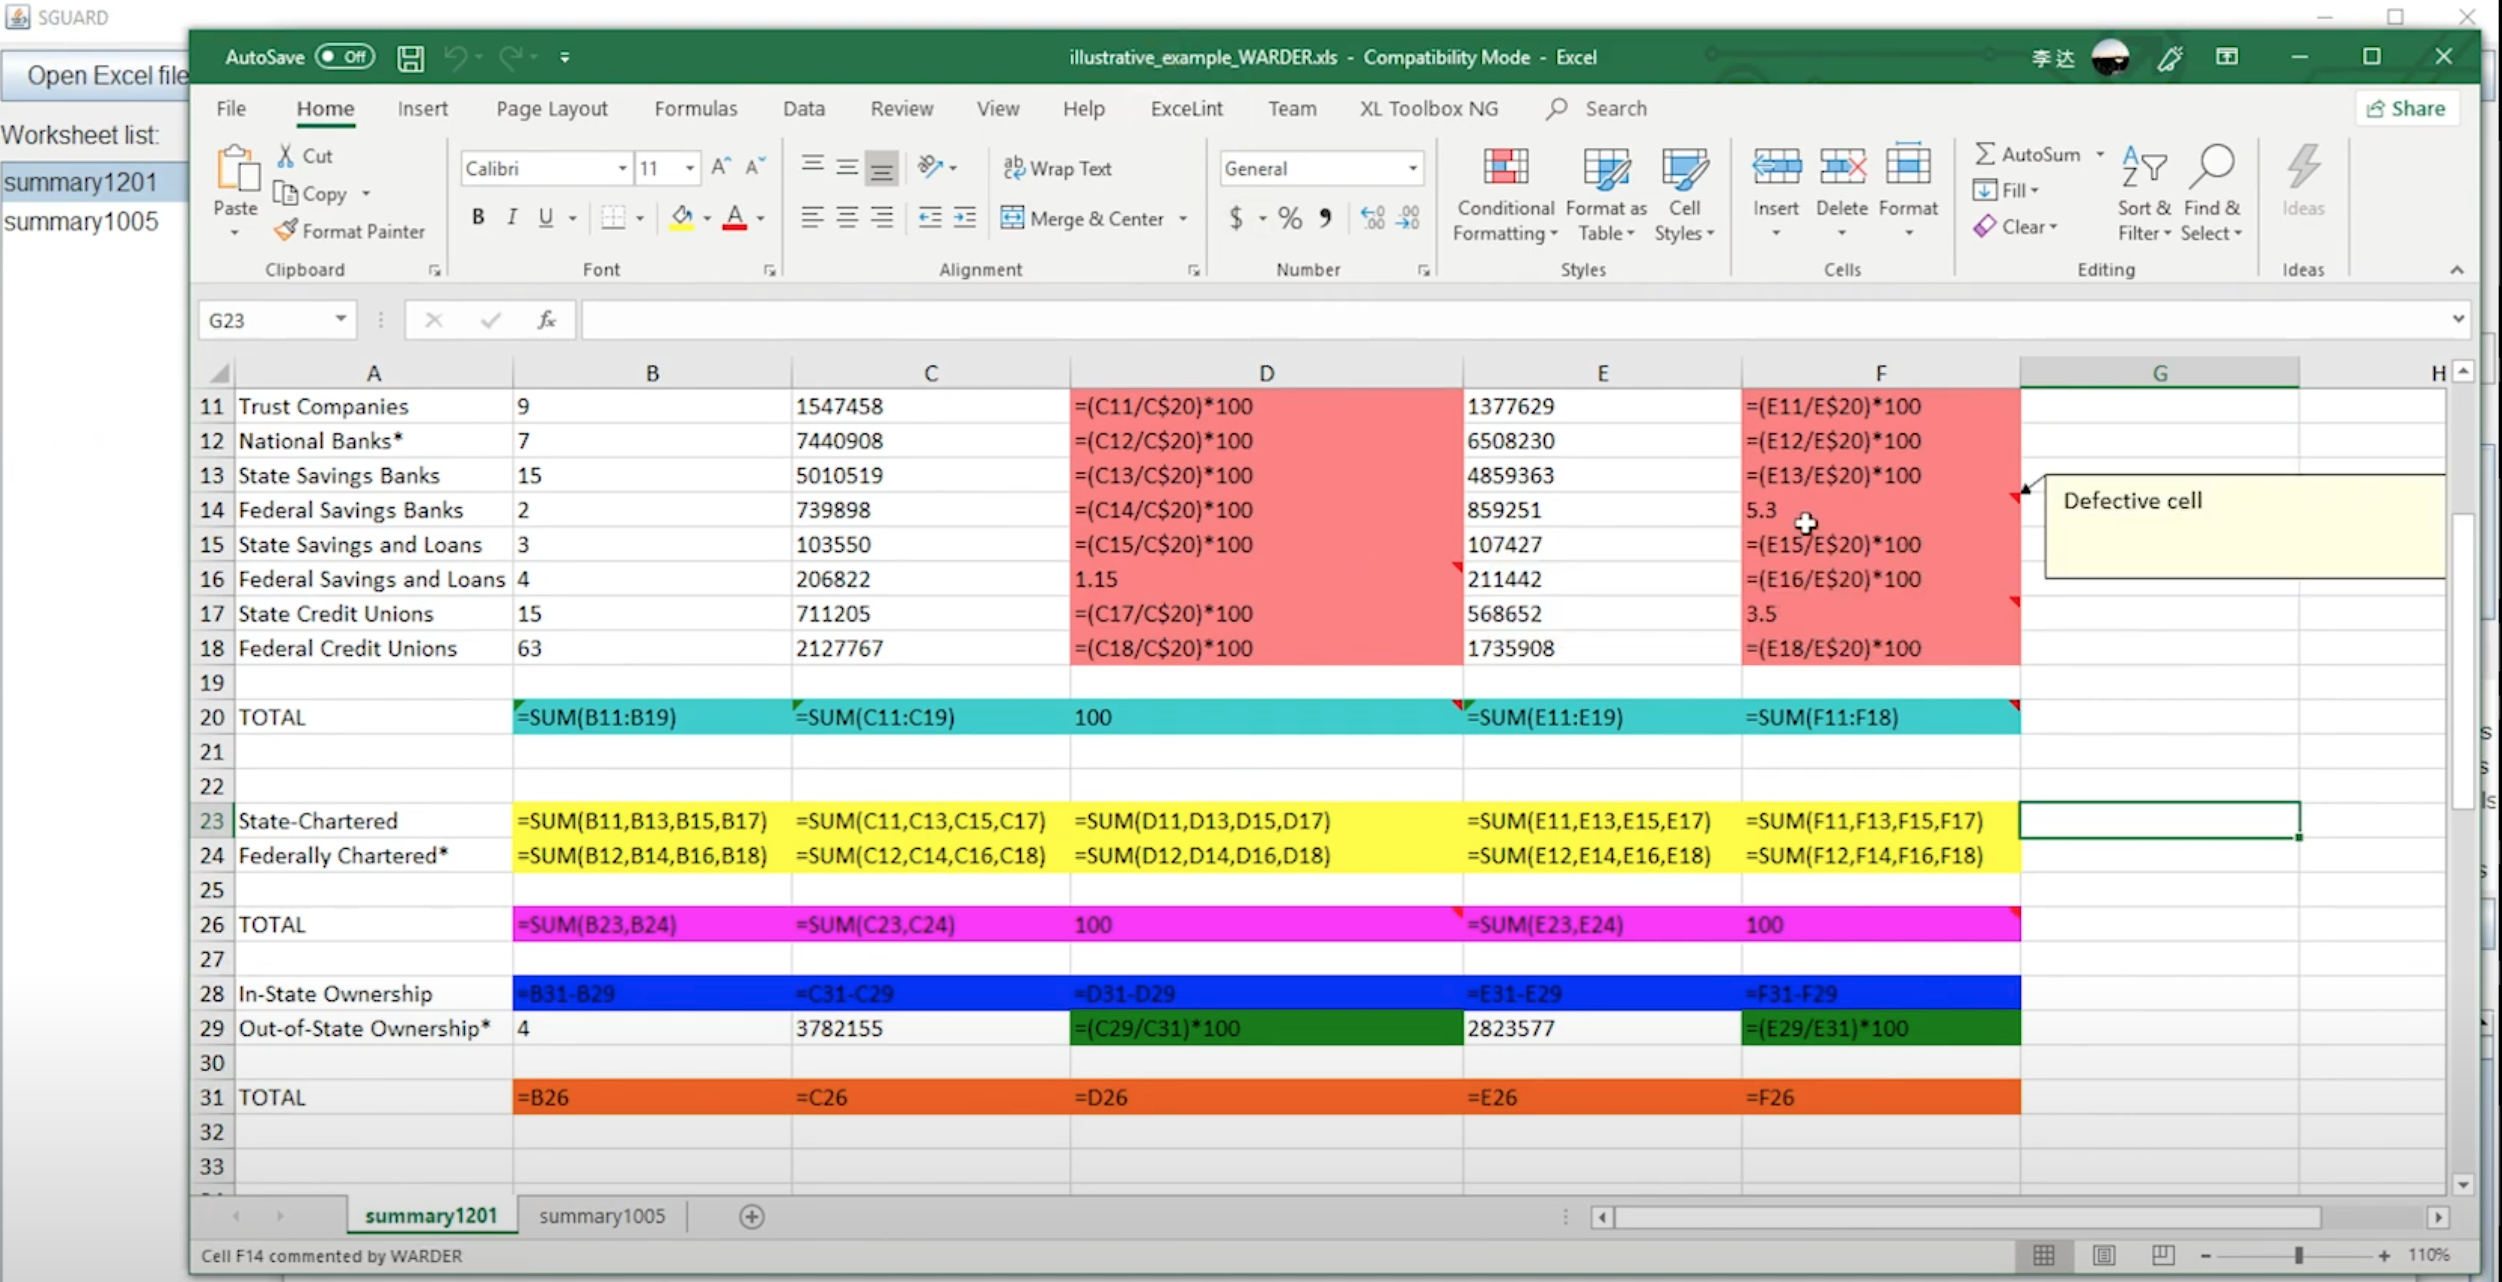
\includegraphics[width=\textwidth]{figure/sg/sguard-8.png}
    \caption{在 Excel 中查看保存好的 \wa 检测结果}
    \label{figure-sg8}
\end{figure}

\begin{enumerate}
    \item 如图\ref{figure-sg1}和\ref{figure-sg2}所示,我们点击 Open Excel file 按钮,从文件浏览器中选择一个要测试的电子表格,这里我们选择预先写好的 illustrative\_example.xls 文件;
    \item 如图\ref{figure-sg3}所示,从左侧列出的工作表中,我们选择名为 summary1201 的工作表,对应的单元格内容就自动显示在正中间;
    \item 如图\ref{figure-sg4}所示,我们在右侧功能区选择准备使用的电子表格测试技术,这里我们勾选上出TableCheck 之外的所有技术,并点击 Start analysis 开始执行;
    \item 如图\ref{figure-sg5}所示,我们会在 Logs 区域看到各个技术开始和结束的标志,在 Defective cells 选项卡里可以勾选上多个技术,查看对应检测到的缺陷单元格全集,这里我们仅选择\wa 技术,可以看到\wa 检测到了 7 个缺陷单元格,与 Info 区域显示的检测结果保持一致;
    \item 类似地,如图\ref{figure-sg6}所示,我们在 Marked clusters 选项卡里可以勾选多个技术,这里我们仅选择\wa 技术,中间区域就显示出\wa 检测到的 7 个单元格类,与 Info 区域显示的检测结果保持一致;
    \item 如图\ref{figure-sg7}所示,我们点击 Save to files 按钮之后,每个技术的检测结果单独生成一个 Excel 文件,和源文件放在同一个目录下;
    \item 如图\ref{figure-sg8}所示,我们点开任意一个工具标注的 Excel 文件,这里我们打开 illustrave\_example\_WARDER.xls 文件,该文件中标注了和 \sg 工具中显示的相同的单元格类,以及在右上角用注释的方式标注出有缺陷的单元格。
\end{enumerate}


%% TODO: hurry
\section{\eg 插件测试工具}

\eg 插件测试工具使用 JavaScript 语言实现,可在 Excel 软件中直接加载并使用的第三方插件,采用 Microsoft 公司开发的 Office-js \footnote{https://github.com/OfficeDev/office-js} 框架来异步读写和操作 Excel 文件。比\sg 更好地是,只要是 Excel 可以运行的平台,如 Windows,MacOS或者浏览器中,都可以加载我们的\eg 插件,接近于跨平台兼容(暂不支持 Linux 操作系统,因为 Excel 本身就没有 Linux 发行版,未来可能考虑开发和 LibreOffice 兼容的 Linux 版本的 \wa 测试工具)。相应的工具源码发布在 GitHub 上\footnote{https://github.com/dlee992/EGuard}。

\eg 测试工具的完整实现包含 \dots 行 JavaScript 代码,其中包含 \dots 行核心功能代码和 \dots 行图形界面代码。

\subsection{界面设计}

如图所示,\eg 使用 Excel 中嵌入一个网页的方式来和用户交互,进行电子表格单元格聚类和缺陷检测的测试过程。
整个交互界面分为如下部分:
\begin{enumerate}
    \item 上方 
    \item 中间 
    \item 下方 
\end{enumerate}

\subsection{使用展示}

接下来,我们结合一个简单的工作表例子来展示\eg 的完整使用流程。